\documentclass[10pt]{article}
\usepackage[margin=20mm]{geometry}
\usepackage{amsmath,amssymb,booktabs,tikz,graphicx,hyperref,xurl}
\hypersetup{colorlinks=true,urlcolor=blue}
\title{Exact finite buffers for the actual rational-kernel inverse}
\author{Producer proof report; unsigned PCC standing}
\date{8 November 2026}
\begin{document}\maketitle
The coefficientwise inverse now has a finite modular-buffer specification
connected to the actual source denominator. It no longer assumes that a caller
supplies a full approximation and its exact inverse. All statements below have
\texttt{[pcc:unverified]} standing pending a trusted independent signature.
No new experiment or benchmark was run.

\section*{Exact coefficient precision}
Let $A=\{r\in\mathbb Q:|r|_2\le1\}$. For every commutative ring $R$, scalar
$c\in R$, jet length $q$ and series $f$,
\[f\in(C(c),X^q)\quad\Longleftrightarrow\quad
 c\mid[X^n]f\ \text{for every }n<q.\]
\texttt{FiniteBuffers.jet\_mem\_iff\_coeff\_divisible} proves both directions.
For the reverse implication it constructs the coefficient witnesses, then
factors the remainder by $X^q$. There is no nonzero-scalar, domain or
completeness assumption.

\texttt{buffer\_eq\_iff\_jet} specializes this to $c=2^p$ over $A$:
two length-$q$ coefficient vectors in $A/(2^p)$ agree exactly when their
series differ by the actual jet ideal $(2^p,X^q)$. Claim
\texttt{PCC-20261108-ff4290} pins the statement.

\section*{Finite inverse constructor}
\texttt{liftBuffer} zero-extends a vector indexed by $\operatorname{Fin}q$.
\texttt{invertBuffer} takes that vector and its known constant unit, applies
the standard inverse coefficient recurrence, and returns the first $q$
coefficients. For the actual denominator $D$, the genuine mapped source unit
$\rho_m$ has the required constant value. The case $q=0$ is the unique empty
vector.

\texttt{actual\_invertBuffer\_correct} proves equality to the actual inverse
buffer. It does not ask the caller for full series $E,F$ with $EF=1$; the
proof constructs them internally from the finite input. The general
low-coefficient lemma explains why input coefficients at or above $q$
cannot affect the returned coefficients. Claim
\texttt{PCC-20261108-24cbda} includes this actual-source scope.

\section*{Concrete modular encoding}
The restriction of the standard two-adic residue map gives a ring map
$A\to\mathbb Z/2^p\mathbb Z$. \path{ResidueEncoding.residue_kernel}
proves its kernel is exactly $(2^p)\subset A$. Surjectivity and the first
isomorphism theorem give the actual ring equivalence
\[A/(2^p)\ \simeq\ \operatorname{ZMod}(2^p).\]
\texttt{residue\_formula} identifies this map with
\[r\longmapsto\operatorname{num}(r)\operatorname{den}(r)^{-1}\pmod{2^p}.\]
The denominator is proved to be a unit from the actual norm bound; no
p-adic approximation oracle is required to use the formula.
\texttt{modular\_inverse\_correct} proves the finite operator correct in
this modular encoding for every actual source scale/node and every $p,q$.

\newpage
\section*{Proof chain and representation scope}
\begin{center}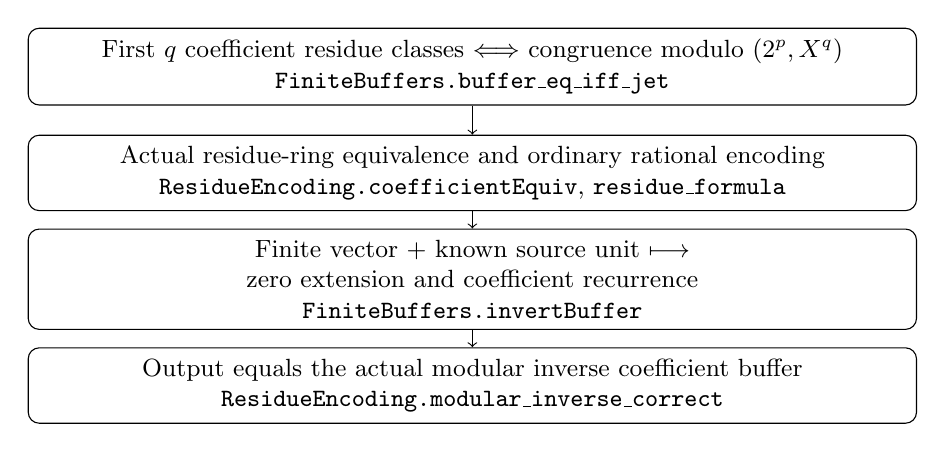
\begin{tikzpicture}[every node/.style={draw,rounded corners,align=center,text width=11cm,font=\small,inner sep=4pt},node distance=1.35cm]
\node (a) {First $q$ coefficient residue classes $\Longleftrightarrow$ congruence modulo $(2^p,X^q)$\\\texttt{FiniteBuffers.buffer\_eq\_iff\_jet}};
\node[below of=a] (b) {Actual residue-ring equivalence and ordinary rational encoding\\\texttt{ResidueEncoding.coefficientEquiv}, \texttt{residue\_formula}};
\node[below of=b] (c) {Finite vector + known source unit $\longmapsto$ zero extension and coefficient recurrence\\\texttt{FiniteBuffers.invertBuffer}};
\node[below of=c] (d) {Output equals the actual modular inverse coefficient buffer\\\texttt{ResidueEncoding.modular\_inverse\_correct}};
\draw[->](a)--(b);\draw[->](b)--(c);\draw[->](c)--(d);
\end{tikzpicture}\end{center}
\texttt{modular\_buffer\_card} proves exactly $2^{pq}$ possible length-$q$
modular vectors. This is an information/cardinality statement, not a measurement
of a program's allocation. Claim \texttt{PCC-20261108-ffec83} records the
ring equivalence, residue formula and cardinality.

The current Lean operator uses mathematical structures marked noncomputable.
The residue formula supplies its ordinary finite arithmetic interpretation,
but these proofs do not certify a compiler, a native implementation or a
bit-operation bound. Such claims require a separate refinement and cost proof.

\section*{Verification and provenance}
The mathematical source is in \path{lean/FiniteBuffers.lean} and
\path{lean/ResidueEncoding.lean}; source commit \texttt{07cfb5586} contains
them. The default Lake build includes both modules. The actual expanded
source gate checks transitive axioms; the official import-inclusive fresh
replay and status receipts are recorded in
\path{lean/FINITE_BUFFERS_VERIFICATION.md}. All failed elaborations remain
in the evidence directory, not accepted as proofs. No checker, kernel or
trust list was changed.

The original empirical protocol, instrument, raw data, export, plots and PDFs
remain unchanged. This is a new versioned proof report. No additional panel,
timing run or cloud job occurred. The current main merge preserves both
appended session logs; the PCC main-prefix check passes without rewriting
events.

CI caught missing declaration hashes in unsigned claim metadata. The original
records are archived; canonical pins and corrected registrations were appended.
No theorem, verifier or trust policy changed. See \path{pcc-pin-repair/}.

Sources checked: the pinned Mathlib power-series coefficient and
$X$-divisibility APIs, ideal-span/quotient APIs, PadicInt residue maps and
kernel, rational denominator unit, and ZMod inverse/cardinality APIs. KB
queries were unavailable (status127); primary-source fallback, no priority
or literature-exhaustion claim.

\section*{The remaining asymptotic obligation}
The local finite representation is now explicit. The outstanding obligations
are actual contraction homogeneity, full finite-precision Hermite recovery,
and uniform all-level modes with construction and child-call bit costs.
These local algebraic statements neither supply nor bound that complete
recursive algorithm. See \path{PLAN.md}; no sub-exponential algorithm theorem
or unrestricted nonexistence theorem is asserted by this report.
\end{document}
